\chapter{Implementación}

\section{Descripción de la implementación}

A diferencia de enfoques anteriores que analizan todas las señales médicas como una única entrada conjunta, en este trabajo se propone una estrategia basada en la exploración de relaciones específicas entre variables fisiológicas. En lugar de tratar el conjunto de signos vitales como una entidad monolítica, se opta por aplicar un modelo de detección de anomalías a cada pareja de señales disponible. Es decir, se estudia cada combinación posible de dos señales fisiológicas como un subespacio independiente, lo que permite estudiar la forma en que se relacionan y evolucionan conjuntamente esas dos señales a lo largo del tiempo, capturando interacciones que pueden reflejar cambios fisiológicos relevantes en el estado del paciente.

Concretamente, se analizan las parejas máximas (\textit{max pairs}) formadas a partir del conjunto total de signos vitales disponibles. Este concepto se refiere al número máximo de combinaciones posibles entre dos elementos de un conjunto, considerando todas las posibles parejas únicas sin repetición. Por ejemplo, si se cuentan con $n$ variables fisiológicas, se generan $\frac{n(n-1)}{2}$ subespacios, cada uno correspondiente a una pareja distinta. Cada uno de estos subespacios es procesado individualmente por el modelo de detección de anomalías basado en \textit{Hierarchical Temporal Memory }(HTM), lo que permite identificar patrones anómalos en la evolución conjunta de las dos señales fisiológicas a lo largo del tiempo.

\section{Descripción del modelo}

El modelo propuesto se basa en la arquitectura de \textit{Hierarchical Temporal Memory} (HTM), que es un enfoque inspirado en el funcionamiento del cerebro humano. HTM es particularmente adecuado para el análisis de datos temporales y secuenciales, lo que lo convierte en una opción ideal para el estudio de señales fisiológicas que varían con el tiempo.

El procesamiento de señales fisiológicas continuas plantea diversos desafíos intrínsecos que resulta dificil de manejar con modelos convencionales. Uno de los principales desafios es la presencia de ruido y artefactos. Esto se debe a que las señales biomédicas frecuentemente se ven contaminadas por interferencias eléctricas, movimientos del paciente o limitaciones de los propios sensores. Esto significa que los datos crudos pueden contener picos o fluctuaciones que no reflejan un cambio real en el estado del paciente, sino meras perturbaciones. HTM aborda esta dificultad gracias a su capacidad para aprender patrones temporales robustos. Al aprender la estructura temporal normal de la señal, el modelo puede identificar y tolerar cierto nivel de ruido, ya que estos no suelen formar parte de las secuencias coherentes aprendidas, permitiendo que el sistema se enfoque en desviaciones persistentes y significativas del comportamiento normal.

Otro desafío importante es la detección de anomalías sutiles y de evolución lenta. No todas las condiciones críticas se manifiestan como cambios abruptos y evidentes en las señales. Algunas pueden comenzar como desviaciones pequeñas y graduales de la normalidad que, si bien individualmente pueden parecer insignificantes, acumuladas en el tiempo indican un problema emergente. Los métodos que se basan en umbrales fijos o que solo analizan signos vitales aislados pueden pasar por alto estas señales de alerta tempranas. La fortaleza de HTM en este aspecto radica en su capacidad para aprender y predecir secuencias temporales. Al modelar las dependencias temporales en los datos, HTM puede identificar patrones anómalos que se desarrollan a lo largo del tiempo, incluso si las desviaciones en cada punto individual son pequeñas \parencite{AHMAD2017134}
\medskip

\section{Flujo de datos en la arquitectura propuesta}

La figura~\ref{fig:arquitectura_subespacios} ilustra el flujo de datos en la arquitectura propuesta para emplear modelos HTM en el análisis de señales médicas en subespacios. A continuación se describen con detalle las cuatro secciones que componen el flujo de datos:

\begin{figure}[ht]
  \centering
  \includesvg[width=\textwidth, inkscapelatex=false]{Images/ArquitecturaSubespacios.svg}
  \captionsetup{justification=centering}
  \caption{Arquitectura de análisis de señales médicas mediante modelos HTM independientes por pareja de signos vitales.}
  \label{fig:arquitectura_subespacios}
\end{figure}

\subsubsection*{Capa de Entrada de Datos: Procesamiento de Signos Vitales}

En la primera etapa de entrada de datos se envían los valores de los diferentes signos vitales procedentes de los dispositivos de monitoreo clínico. Cada par de señales corresponde a un subespacio independiente de análisis. Por ejemplo, \emph{(FC, SpO\textsubscript{2})} constituye un primer subespacio, \emph{(FC, Resp)} un segundo, y así sucesivamente hasta cubrir todas las parejas máximas posibles.

En este trabajo, los datos se obtienen como resultado de exportar las lecturas de signos vitales de un paciente, registradas segundo a segundo en un archivo, lo que permite disponer de un registro detallado y continuo para su posterior análisis. Particularmente, la información que se dispone por cada signo vital disponible es:

\begin{itemize}
  \item Serie temporal de cada señal, con su correspondiente marca de tiempo.
  \item Identificador del paciente y etiqueta de tipo de señal, de modo que cada registro quede correctamente asociado a su fuente original.
  \item Edad del paciente, que debe ser ingresada manualmente por las enfermeras al inicio del monitoreo.
\end{itemize}

\bigskip

\subsubsection*{Capa de Detección de Anomalías: Modelos HTM por cada subespacio}

En esta sección, cada pareja de señales se envía a un modelo HTM independiente. Cada modelo HTM recibe como entrada la serie temporal correspondiente y ejecuta las siguientes operaciones, repitiendo este proceso para cada instante temporal registrado.

\begin{enumerate}
  \item \textbf{Codificación Temporal}: Convierte las lecturas numéricas de ambas señales de entrada en una representación binaria, adecuada para el procesamiento jerárquico de HTM.
  \item \textbf{Aprendizaje No Supervisado}: el modelo HTM actualiza progresivamente su estructura conforme recibe nuevos vectores de entrada, de modo que aprende los patrones temporales normales de dicha pareja de señales.
  \item \textbf{Cálculo de Puntuación de Anomalía}: para cada nueva muestra, el modelo HTM calcula un valor escalar entre 0 y 1 que refleja el grado de desviación con respecto al comportamiento aprendido hasta el momento. Se considera que este dato es anómalo si la puntuación supera un umbral predefinido, lo que indica que la pareja de señales presenta un comportamiento inusual en ese instante temporal.
\end{enumerate}

Adicionalmente, al contar con la edad del paciente, cada subespacio tiene la capacidad de ajustar el resultado del modelo en función de los rangos fisiológicos normales para ese grupo etario. Dado que en este enfoque se considera una anomalía como cualquier cambio significativo en la pareja de signos vitales analizada, es posible que el modelo detecte como anómalo un momento en el que el paciente transiciona rápidamente hacia un estado de recuperación, donde todos sus signos vitales se encuentran dentro del rango normal. Esto puede resultar en un falso positivo, ya que el modelo identifica una desviación respecto a la secuencia previa, aunque el nuevo estado sea clínicamente deseable. Para evitar este tipo de falsas alertas, cada subespacio puede decidir ignorar una anomalía si, en el instante considerado, ambos signos vitales de la pareja se encuentran dentro de los valores normales definidos para la edad del paciente. De este modo, se mejora se reduce la generación de alertas innecesarias y se espera mejorar la confiabilidad del sistema.

Por otra parte, ya que definimos una anomalía como una alteración en el comportamiento de dos o más signos vitales, no podemos considerar como anómalo un momento en el que la lectura de alguno de los signos vitales se vea interrumpida. Por lo tanto, si una de las señales de la pareja no está disponible en un instante temporal, el modelo HTM no genera una puntuación de anomalía para ese momento. Esto permite que el sistema pueda manejar situaciones en las que uno o más signos vitales no estén disponibles sin generar alertas erróneas.

Cada modelo HTM envía a la siguiente capa (generación de alertas) la siguiente información:

\begin{itemize}
  \item \emph{Identificador de la pareja de señales} analizada (por ejemplo, “FC, SpO\textsubscript{2}”).
  \item \emph{Marca de tiempo} que acompaña a la muestra de entrada.
  \item \emph{Resultado de la puntuación de anomalía}, que es un valor entre 0 y 1, donde 0 indica normalidad y 1 indica una anomalía extrema.
  \item \emph{Confianza del modelo}, que es un valor entre 0 y 1 que indica la certeza del modelo sobre la puntuación de anomalía calculada.
\end{itemize}

\bigskip

\subsubsection*{Capa de Generación de Alertas: Cálculo del Nivel de Alerta del Paciente}

La capa de generación de alertas consiste en una composición de los resultados obtenidos en cada subespacio con el fin de determinar el nivel de alerta de un paciente en un instante dado. Para ello, se calcula primero el \emph{nivel de criticidad} de cada subespacio, definido como el producto entre:

\begin{itemize}
  \item $\delta_i \in \{0,1\}$: indicador binario que toma valor 1 si el modelo detectó una anomalía en el $i$-ésimo subespacio, y 0 en caso contrario.
  \item $c_i \in [0,1]$: confianza otorgada por el modelo HTM para la puntuación de anomalía en el $i$-ésimo subespacio.
\end{itemize}

A partir de estos niveles de criticidad individuales, definimos la criticidad global del paciente en el instante $t$ como la suma de los niveles de criticidad de todos los subespacios que han entregado un resultado válido. Formalmente:

\[
  C(t) \;=\; \sum_{i \,\in\, \mathcal{A}(t)} \bigl(\delta_i \cdot c_i \bigr),
\]

donde $\mathcal{A}(t)$ es el conjunto de índices de subespacios activos en el instante $t$ (es decir, aquellos que han entregado un resultado válido y no presentan interrupciones en la lectura de los signos vitales). Sin embargo, puesto que puede ocurrir que algunos subespacios no entreguen respuesta en un instante dado, debido a desconexiones o interrupciones en la lectura de los signos vitales, es necesario normalizar esta suma entre el número de subespacios activos. De esta forma, el \emph{nivel de alerta} del paciente en el instante $t$ se define como:

\[
  C(t)
  \;=\;
  \frac{
    1 + \displaystyle\sum_{i \,\in\, \mathcal{A}(t)} \bigl(\delta_i \cdot c_i \bigr)
  }{
    \bigl|\mathcal{A}(t)\bigr|
  }
\]

Supóngase ahora que en un instante dado sólo se obtienen resultados de 3 de los 6 subespacios ($|\mathcal{A}(t)| = 3$). En este escenario, la suma de los niveles de criticidad parciales tendería a subestimar la condición general del paciente debido a la ausencia de datos en los subespacios faltantes. Por esta razón, mediante la normalización entre $\mathcal{A}(t)$, se evita este sesgo, ya que el nivel de alerta se ajusta al número de subespacios activos en ese instante. Esto permite que el sistema mantenga una evaluación más precisa del estado del paciente, incluso cuando algunos signos vitales no están disponibles.

\bigskip

\subsubsection*{Tablero de Control: Visualización Analítica del Estado del Paciente}

En la última sección, el sistema presenta al personal médico un tablero de control que cumple las siguientes funciones:

\begin{itemize}
  \item \textbf{Monitoreo de Signos Vitales}: Muestra, mediante gráficos de series temporales, la evolución simultánea de los diferentes signos vitales.
  \item \textbf{Criticidad del Paciente}: Visualiza de forma destacada el \emph{Nivel de criticidad Actual} junto con las parejas de señales responsables de dicha puntuación. Esto permite al personal médico identificar rápidamente qué combinaciones de signos vitales están contribuyendo al estado crítico del paciente.
  \item \textbf{Generación de Alertas}: Presenta alertas visuales cuando el nivel de criticidad supera un umbral predefinido, lo que indica que el paciente se encuentra en una situación de riesgo.
\end{itemize}

Dado que el índice de criticidad calculado por el sistema se encuentra normalizado en un rango entre 0 y 1, es posible establecer umbrales claros y objetivos para la generación de alertas clínicas. En particular, se propone definir tres niveles de alerta: bajo, medio y alto, en función del valor alcanzado por el indicador de criticidad del paciente. Dicho esto, se considera que el paciente se encuentra en un estado de alerta de nivel bajo cuando el índice de criticidad es inferior a 0.3; si el valor se sitúa entre 0.3 y 0.6, se clasifica como alerta de nivel medio; y cuando el índice supera el umbral de 0.6, se clasifica como una alert de nivel alto, indicando una situación de riesgo significativo que requiere atención inmediata. Esta categorización facilita la interpretación rápida del estado del paciente por parte del personal médico y permite priorizar la respuesta clínica de acuerdo con la gravedad detectada por el sistema.

En la Figura \ref{fig:patient2_dashboard_baja_alerta} se presenta la visualización del tablero de control correspondiente al paciente 2 en un momento en el que el sistema considera que el nivel de alerta es bajo. En la parte izquierda del diagrama se observa claramente qué pareja de signos vitales está participando en la generación de la alerta; por ejemplo, la combinación de frecuencia cardíaca y frecuencia respiratoria muestra una criticidad moderada y mayor influencia en la criticidad del paciente, mientras que la pareja de frecuencia cardíaca y saturación de oxigeno presenta una criticidad baja. Esta visualización permite identificar de manera intuitiva no solo qué signos vitales están involucrados en la generación de cada alerta, sino también la severidad asociada a cada combinación, facilitando la priorización de la atención clínica.

En la parte derecha del tablero se encuentra la evolución temporal de los signos vitales seleccionados, presentada en un gráfico que permite al usuario ajustar fácilmente el periodo de tiempo visualizado. Esta funcionalidad es especialmente útil para analizar tendencias recientes o retrospectivas, apoyando la toma de decisiones informadas por parte del personal médico.

\begin{figure}[ht] \centering 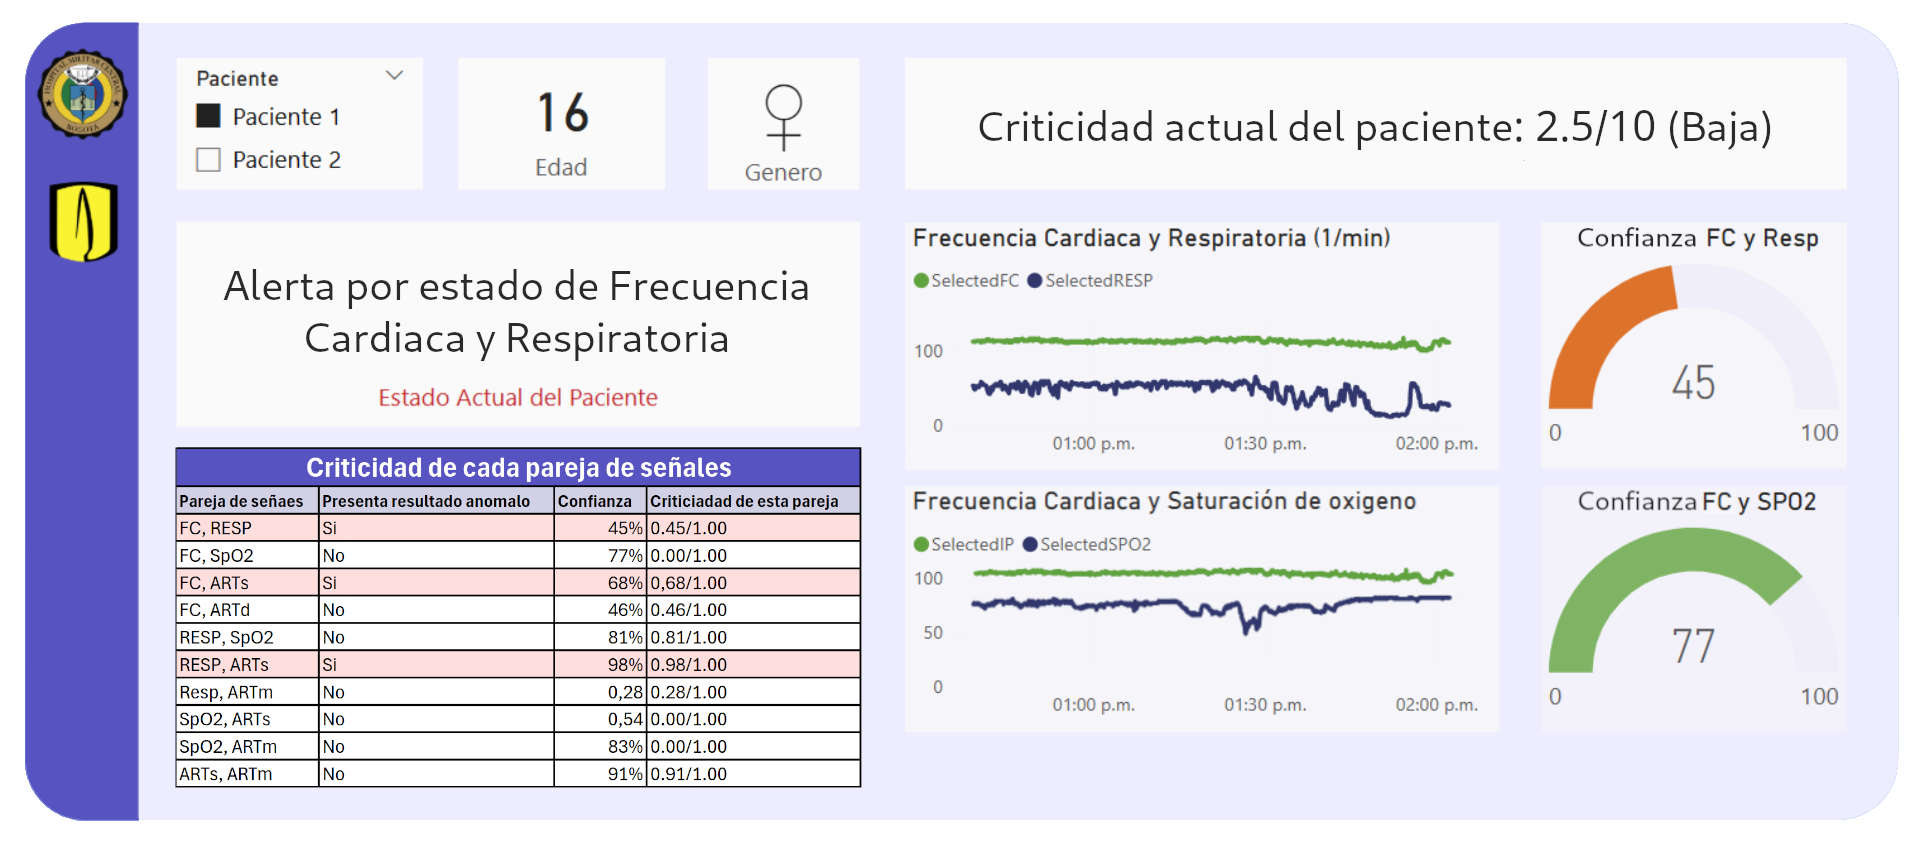
\includegraphics[width=\textwidth]{Images/TableroControl.png} \caption{Visualización del tablero de control para el paciente 2 en estado de alerta baja.} \label{fig:patient2_dashboard_baja_alerta}
\end{figure}

De esta manera, el tablero de control proporciona una visión integral y configurable del estado del paciente, resaltando tanto las combinaciones de signos vitales más relevantes para la alerta actual como la evolución de los parámetros fisiológicos a lo largo del tiempo.